% Appendix 2: The Possibility of Depicting Perceptual Space on a Plane
% Source pages: 247–253

\chapter{The Possibility of Depicting Perceptual Space on a Plane}

\srcpage{247}

The preceding Appendix showed that the system of linear perspective faithfully transmits the
geometry of the retinal image.  As is known (see Chapters\,II and\,III), the system of
perceptual perspective is obtained by transferring the geometric properties of perceptual
space onto the picture plane.  Two questions therefore arise: what are the geometric
properties of that space, and can it be depicted on a plane?

The geometric properties of perceptual space are obtained from the retinal image by
``stretchings'' and ``compressions'' of its elements under the action of the mechanisms of
size constancy and shape constancy.  Speaking of the character of the geometric
transformations associated with these two constancy mechanisms, one immediately sees
their fundamental difference.  The size-constancy mechanism changes the relative sizes of
visible objects depending on their distance from the observer.  Since the only variable on
which the numerical magnitude of the ``stretching'' or ``compression'' depends in this case
is the distance from the observer, one may regard the entire perceived space as subject to
these deformations, independently of which specific objects fill the picture-space.  The
shape-constancy mechanism acts only with respect to a specific object; without deforming
the remaining space, it is tied to that object, and therefore the character of the local
deformation changes when one object is replaced by another.

The system of perceptual perspective must take both effects into account.  Methodologically,
however, it is convenient to consider their action in succession: first the deformation of space
as a whole, then the local deformations associated with the existence of individual objects.
Under this approach one can speak of the system of perceptual perspective in the narrow
sense of the word, in which, when transforming the linear perspective, only the action of the
size-constancy mechanism is taken into account.  Without aiming to find here the specific
regularities of such a perspective system, let us consider the question of whether it is in
principle possible to transfer onto the picture plane the image that arises in human
consciousness---in such a way that the linear dimensions of the perceptual image are
consistent with the linear dimensions of its depiction on the canvas.

Fig.\,2.1 shows the picture plane $KK$, on which the image of the picture-space lying to the
left of $KK$ is obtained in the usual manner of linear perspective---by projecting objects from
some point $B$ located at height $BC$ above the subject plane.  Suppose that, as a result of
the action of the size-constancy mechanism, the apparent size of some object diminishes as it
recedes from the observer less rapidly than one would expect if the apparent size strictly
followed the retinal image.  A small segment $ds$ at point $A$, when projected from~$B$,
will have some characteristic linear size $ds_1$ on the picture plane.  Allowing for the action
of the size-constancy mechanism (and thereby departing from the system of linear
perspective), its image will have size $ds_2 = P\,ds_1$, where $P$~is some function relating
the size of the object as actually perceived by a person to the size that would result if
perception followed strictly from the retinal image.  The function $P$ depends on the distance
of the observed elementary segment from the observer: $l_\Sigma =l_0 + l$.  Since the quantity $l_0$ is
constant, it is convenient to write the function $P$ in the form $P(l)$ or, passing to the
dimensionless variables introduced by relations~(1.1), in the form $P_1(\overline{l})$.

\begin{figure}[H]
    \centering
    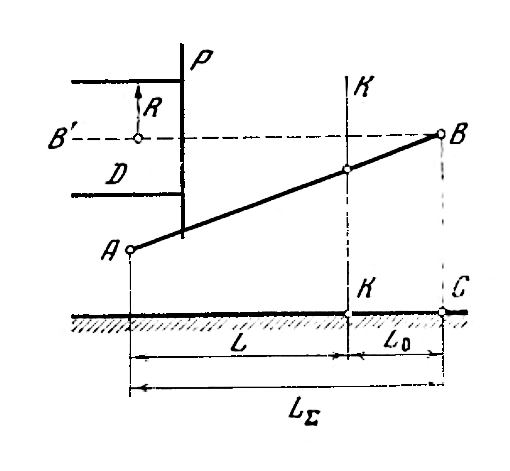
\includegraphics[width=0.5\linewidth]{figures/f2.1.png}
\end{figure}
\figblock{2.1}{Geometry of the perceptual-perspective construction: picture plane $KK$,
  centre of projection $B$ at height $BC$, and the function $P_1(l)$ relating perceptual
  to retinal image sizes.}

It is convenient to begin determining the basic properties of the function $P_1$ by equalising
the scales of the two perspective systems: linear and perceptual.  To this end we assume that
the segment $d\overline{s}$ lies in the picture plane, so $d\overline{s}_1 = d\overline{s}$.  We agree to consider that in the
picture plane (at $b = 0$) the apparent and true sizes coincide, i.e.\ for $l = 0$:
$d\overline{s} = d\overline{s}_1 = d\overline{s}_2$.  Thus for $\overline{l} = 0$, $P_1(0) = 1,$ while for all other distances from the observer. \footnote{For constant $L$ (points at equal
  distance from the picture plane), expression~(2.1) can obviously be written in finite
  form: $x_2 = P_1(L)\,x_1$.}

\srcpage{248}
\begin{equation}
  dx_2 = P_1(l)\,dx_1.
  \tag{2.1}
\end{equation}

In expression~(2.1) the notation has been refined by the transition from $ds$ to $dx$, since
we introduce the assumption that the segment $ds$ is horizontal and parallel to the picture
plane, i.e.\ it coincides with $dx$.

Differentiating equality~(2.1) with respect to $l$, using expression~(1.5) and treating $dx$
as constant:
\begin{equation}
  \frac{d}{dl}dx_2 = \frac{dx}{1+l}\frac{d}{dl}P_1(l) - P_1(l)\frac{dx}{(1+l)^2}
  \tag{2.2}
\end{equation}
where $P_1' = dP_1/dl$.

If one makes the assumption of complete constancy at small distances from the observer
(which is practically always the case), then for sufficiently small $l$ (i.e.\ for a picture
plane sufficiently close to the observer) the size $dx_2$ in the immediate neighbourhood of
the picture plane should not change with increasing~$b$.  Analytically this is expressed by
the condition $\frac{d}{dl}dx_2 = 0$, which on the basis of equality~(2.2) allows one to find a
further condition that the function $P_1(l)$ must satisfy [taking into account the earlier
condition $P_1(0) = 1$]:
\begin{equation}
  \frac{dP_1}{dl}(0)=\left.\frac{P_1(l)}{1+l}\right|_{0} = 1.
  \tag{2.3}
\end{equation}
\vspace{-12pt}
\begin{figure}[H]
    \centering
    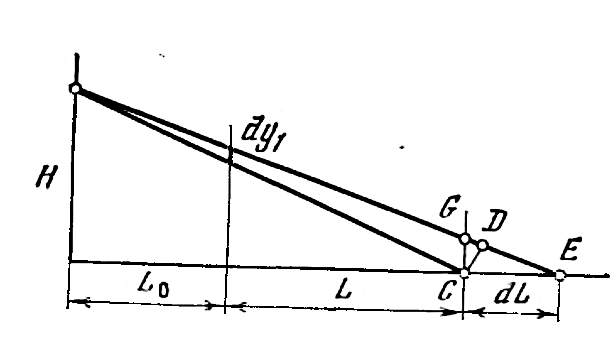
\includegraphics[width=0.6\linewidth]{figures/f2.2.png}
\end{figure}
\figblock{2.2}{Diagram for establishing the relation between the depth increment $dl$ and
  the vertical image increment $dy_1$.}

At $l \to \infty$, i.e.\ at the horizon line, $dx_2 = 0$ regardless of the size of $dx$.  This
is a natural result of the fact that at a sufficiently large distance any object of finite size
will be seen as a point, since its angular size will become so small that it will be able to
excite only a single photoreceptor of the retina.  At $l \to \infty$ the linear perspective
already gives $dx_1 = 0$, and consequently it is sufficient to require that the function
$P_1(\infty)$ be finite, i.e.\ that $P_1(l)$ have a finite upper bound.  Everyday visual
experience testifies to the continuity of the function $P_1(l)$, since, when observing railway
tracks, for example, no one has seen a jump discontinuity in their apparent width at some
distance.  Almost equally evident is the monotonicity of the function $P_1(l)$.  This is
connected with the reasonableness of a uniform response of the human perceptual system
to a uniform stimulus---in the present case, to an increase in distance~$l$.  The monotonicity
of $P_1$ together with the conditions $P_1(0) = 1$ and $dP_1/dl(0) = 1$ allows one to write
$P_1(l) \ge 1$.  Obviously, an infinite family of functions can satisfy the described properties,
and the choice of an appropriate function should be made taking into account experimental
data, the required accuracy, and simplicity of expression in elementary functions.

The function $P_1(l)$ allows one to find the apparent width of element $dx$, or of the road
discussed at the end of the preceding Appendix, if the corresponding image in the system of
linear perspective is known; however, the size-constancy mechanism will change not only
the $x$-coordinate but also~$y$.

Fig.\,2.2 shows the construction enabling one to establish the relation between an increment $dl$ and $dy_1$. 
\begin{equation*}
    dy_1 = \frac{l_0}{l_0+l} \ \frac{H}{l_0+l}dl
\end{equation*}

Differentiating [equation~(1.2)]:
\begin{equation}
  dy_1 = \frac{dl}{(1+l)^2}.
  \tag{2.4}
\end{equation}

\srcpage{249}

The quantity $dy_1$ can be regarded as the image on the picture plane, by the laws of linear
perspective, of a segment $SD$ perpendicular to the line of sight.  The function $P_1(l)$
introduced above transformed some width in linear perspective into another corresponding
to visual perception.  This allows one to transform the image of segment $SD$ by the same
law.  By this assumption the claim is introduced that all segments lying in the plane normal
to the line of sight are transformed by one and the same law: this is natural, for otherwise
the visible image of a flat square normal to the line of sight would, as it recedes from the
observer, transform into a different figure, which no one has observed.  But then
\begin{equation}
  dy_2 = P_1(l)\,dy_1,
  \tag{2.5}
\end{equation}
and consequently, on the basis of equation~(2.4):
\begin{equation}
  y_2 = \int_0^l \frac{P_1(l)}{(1+l)^2}\,dl.
  \tag{2.6}
\end{equation}

Let us return to Fig.\,2.1 and consider the image of some figure lying in the plane~$P$,
parallel to the picture plane $KK$ and located at distance $l_P$ from it.  Since for all
points of plane~$P$, $P_1(l_P) = \mathrm{const}$, the transformation that the image of the
figure undergoes when passing from the linear to the perceptual perspective system will be
a similarity transformation.  Suppose now that in plane~$P$ there lies the rim of an
infinitely extended hollow cylinder~$\Pi$ of radius~$R$ with its axis lying on the line $BB'$.
Then on the picture plane $KK$, under projection from point~$B$ (i.e.\ in the system of
linear perspective), the cylinder will map to a circle centred at the principal point of the
picture, and its infinitely distant end will be represented by that centre.  The image of the
near rim of the cylinder will have radius $r_1 = R\,l_0/(l_0 + l_P) = R/(1+l_P)$.  Let us
ask what the image of this same cylinder will be in the system of perceptual perspective.
Obviously its rim will also appear as a circle centred at the principal point of the picture,
and that centre will simultaneously be the image of its infinitely distant end.  The radius of
the circle representing the near end of the cylinder will be $r_2 = r_1 P_1(l_P)$, and the
image of the cylinder's generator receding to infinity, on the picture plane in the system of
perceptual perspective, will by equality~(2.6) have size\footnote{Not shown in the figure.}

\srcpage{250}
\begin{equation}
  l_2 = \int_{l_P}^{\infty} \frac{P_1(l)}{(1+l)^2}\,dl.
  \tag{2.7}
\end{equation}

Let us compare $l_2$ and $r_2$.  With the expression for $r_1$:
\begin{equation}
  r_2 = \frac{R\,P_1(l_P)}{1+l_P}.
  \tag{2.8}
\end{equation}

If one were to assume that under the integral sign in~(2.7) stood not $P_1(l)$ but the
constant value $P_1(l_P)$, it would be easy to verify that $l_2 = r_2$.  Since, however, for
$l > l_P$ the monotonically increasing character of $P_1(l)$ gives $P_1(l) > P_1(l_P)$, it
is evident that
\begin{equation}
  l_2 > r_2.
  \tag{2.9}
\end{equation}

The inequality obtained shows the in-principle impossibility of depicting the considered
cylinder in the system of perceptual perspective.  Indeed, the image of the cylinder's
generator must have one end at the image of the infinitely distant point---i.e.\ at the centre
of the circle of radius~$r_2$---and the other end on that circle.  Since from point~$B$ only
the inside of the cylinder is visible, all points of the image of its surface must lie inside the
circle of radius~$r_2$.  But since $l_2 > r_2$, the images of the near ends of the generators
will not lie on the circle but will fall outside it, which is impossible as it contradicts the
preceding condition.

As is known, to prove some proposition one must show that it holds always, while to refute
it, it suffices to give a single counter-example.  The considered example of depicting a
hollow cylinder therefore refutes the view (if it existed) that the perceptual perspective
system is capable of serving as a representation of any body.  In contrast, the system of
linear perspective, which reduces to projecting from point~$B$ objects in the picture-space,
is capable of transmitting the projection of any object onto the picture plane (although for
large visual angles this formally correct image will convey the visual impression in a
strongly distorted form).

The in-principle inability of the perceptual perspective system to represent any arbitrary
object on the picture plane requires the identification of the class of objects whose
depiction in the system of perceptual perspective is possible.  The monotonically increasing
function $P_1(l)$ has a finite upper bound, which leads to the practical constancy of $P_1(l)$
starting from some sufficiently large value of~$l$.  But then for the distant regions of space
the image in the perceptual perspective system is similar to the image in the linear
perspective system, i.e.\ always possible.  In exactly the same way, figures lying in planes
parallel to the picture are depictable; as noted above, they are obtained from the linear
perspective system by a similarity transformation.

Let us finally give one more case---the depiction of a comparatively narrow portion of a
plane parallel to the axis $BB'$.  Such a portion, even if it begins at the picture plane and
has infinite extent in depth, can be consistently depicted on the picture plane, since its
transformations (which, as is evident from the foregoing, have the character of stretching)
in the ``receding'' direction and in the lateral direction are independent.  By virtue of this
independence, the occurrence of a contradiction of the kind discussed in connection with the
cylinder is impossible (in the above example, the quantity~$l_2$, directed ``away from the
observer'', and the quantity~$r_2$, directed laterally, were linked by the unfulfilable
requirement $r_2 = l_2$).

\srcpage{251}

Thus the depiction of nearby portions of planes parallel to the picture, perpendicular to it,
and horizontal, in the system of perceptual perspective is possible.  Precisely such portions
of planes most frequently occur in depicting various rectangular objects.  Since, by what has
been said, the depiction of such portions is feasible, one should consider whether the
perceptual perspective system can be used to represent the spatial objects composed of them.
Let us consider in this connection two typical cases.

\smallskip
\textit{Case~I.  Depiction of an interior (a parallelpiped seen from inside).}
Fig.\,2.3 shows the projection of some interior onto the picture plane, i.e.\ its image in the
system of linear perspective.  Let the bounding rectangle have area~$S_1$; this rectangle
represents the cross-section of the parallelpiped closest to the observer---as it were, the
``entrance'' to the interior.  Let this section correspond to some value $l = l_P$, while all
other planes bounding the interior-space will naturally lie at $l > l_P$.  Write the obvious
identity
\begin{equation}
  S_1 = \iint_{s_1} dx_1\,dy_1,
  \tag{2.10}
\end{equation}
which gives the area of the ``entrance'' in the system of linear perspective.

On the basis of relations~(2.1) and~(2.5), $dx_2\,dy_2 = P_1^2(l)\,dx_1\,dy_1$.  Then
\begin{equation}
  S_2 = \iint_{s_1} P_1^2(l)\,dx_1\,dy_1,
  \tag{2.11}
\end{equation}
where $S_2$ is the area bounded by the contour of the image in the system of perceptual
perspective.

\begin{figure}[H]
    \centering
    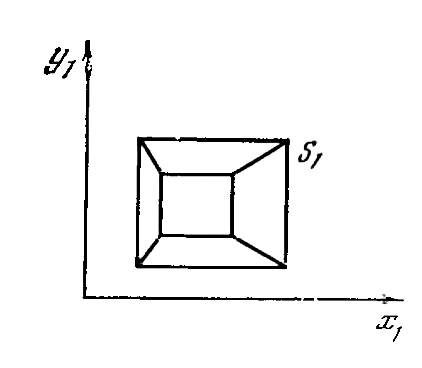
\includegraphics[width=0.3\linewidth]{figures/f2.3.png}
\end{figure}
\figblock{2.3}{Projection of an interior (parallelpiped seen from inside) onto the picture
  plane in linear perspective.  The outer contour serves simultaneously as the boundary of
  the ``entrance'' plane and of the walls, floor, and ceiling.}

However, the outer contour of the interior shown in Fig.\,2.3 has two meanings: first, it
bounds the image of the ``entrance'' plane, and second, it bounds the images of the walls,
floor, and ceiling.  In the first case the perceptual image should correspond to the area
\begin{equation}
  S_2' = P_1^2(l_P)\iint_{s_1} dx_1\,dy_1 = P_1^2(l_P)\,S_1,
  \tag{2.12}
\end{equation}
and in the second to the area
\begin{equation}
  S_2'' = \iint_{s_1} P_1^2(l)\,dx_1\,dy_1,
  \tag{2.13}
\end{equation}

\srcpage{252}

where the values of $l$ are taken for the corresponding boundary points of the interior.  By
virtue of the properties of $P_1(l)$ stated above and the fact that in the case under
consideration $l > l_P$, one obtains the inequality
\begin{equation}
  S_2'' > S_2',
  \tag{2.14}
\end{equation}
which, like inequality~(2.9), testifies to the impossibility of depicting an interior in the
system of perceptual perspective, even though each wall, floor, and ceiling individually
can be depicted.

\begin{figure}[H]
    \centering
    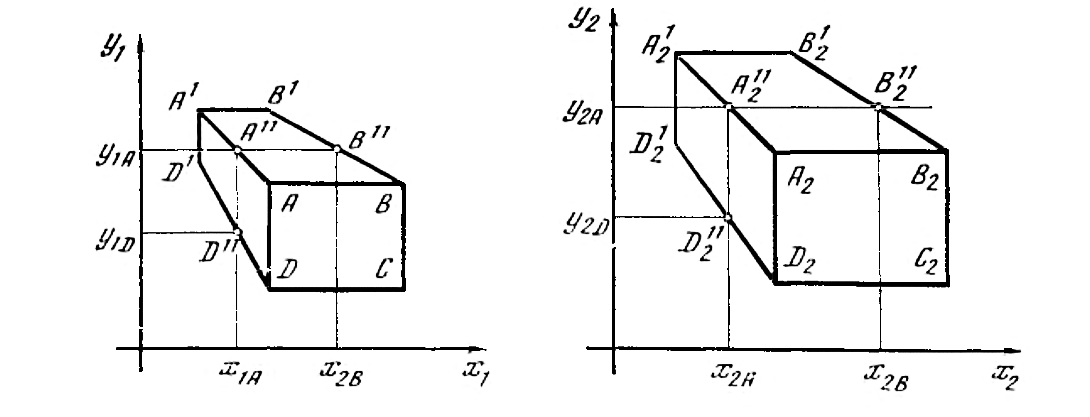
\includegraphics[width=0.8\linewidth]{figures/f2.4.png}
\end{figure}
\figblock{2.4}{The same parallelpiped shown twice: left in linear perspective, right in
  perceptual perspective.  The perceptual image of the nearest face is enlarged by factor
  $P_1(l_P) > 1$; lateral faces undergo a more complex transformation.}

\textit{Case~II.} Depiction of a parallelpiped with faces parallel to the coordinate planes, seen from outside. Fig.\,2.4 shows such a depiction twice: on the left in the system of linear perspective, on
the right in the system of perceptual perspective.  Let the face of the parallelpiped nearest
to the observer be at distance $l_P$ from the picture plane.  Since the passage to the
perceptual image, as already noted, involves for such planes a similarity transformation, the
perceptual image of face $A_2B_2C_2D_2$ will differ from the face $ABCD$ obtained by
central projection only in scale---it will be larger, since $P_1(l_P) > 1$.  The lateral
faces $ABB'A'$ and $ADD'A'$ will be transformed in a more complex manner, since the
function $P_1(l)$ will not be constant for them.  Let the $y$-axis be the trace of the section
of the picture plane by the vertical plane passing through the centre of projection and
containing the line perpendicular to the picture plane.  Then for each given $l = l_1$:
\begin{equation}
  y_{1A} = H - \frac{H_1}{1 + l_1},
  \tag{2.15}
\end{equation}
where $H$ is the height of the viewpoint and $H_1$ is the distance from the centre of
projection to the plane containing face $ABB'A'$.

The horizontal line $y_1 = y_{1A}$ will intersect the image of face $ABB'A'$ at points $A''$
and $B''$.  The image shown on the right of the parallelpiped can be constructed as follows.
Let the image of edge $A_2A_2'$ already be built in one way or another.  Taking the
point~$A_2$ on it corresponding to~$A''$, and drawing a horizontal line through it, lay off
on it the distance determining the position of point~$B_2$ corresponding to~$B''$:
\begin{equation}
  x_{2B} - x_{2A} = \bigl(x_{1B} - x_{1A}\bigr)\,P_1(l_1),
  \tag{2.16}
\end{equation}
and the vertical segment
\begin{equation}
  y_{2A} - y_{2D} = \bigl(y_{1A} - y_{1D}\bigr)\,P_1(l_1),
  \tag{2.17}
\end{equation}
measured from point~$A_2$, will determine the position of the corresponding point.

In such a construction no manifest contradictions arise [of the type of relations~(2.9)
and~(2.14)], since the construction of points $B_2$ and $D_2$ is independent (directed in
``different directions'') and not bounded by any conditions.

Nevertheless, the resulting image will carry a distortion of the visual impression.  One can
show that the found distance of point~$D_2$ from the horizontal through~$A_2$, and its
distance from the horizontal through~$D_2$ (obtainable by starting the construction
directly from~$D_2$ rather than via~$A_2D_2B_2$), will turn out to be inconsistent---they
will not sum to the distance between $A_2B_2'$ and $D_2C_2$.  This is further aggravated
by the already noted impossibility, discussed in Chapter~III, of an image correctly
transmitting the three simultaneously visible angles at a vertex of a parallelpiped.  Thus a
flawless depiction of a parallelpiped ``from outside'' is likewise impossible, although the
errors thereby arising are less conspicuous.

%\srcpage{253}
